\documentclass[../main/report.tex]{subfiles}
\begin{document}
\begin{figure}[H]
	\centering
	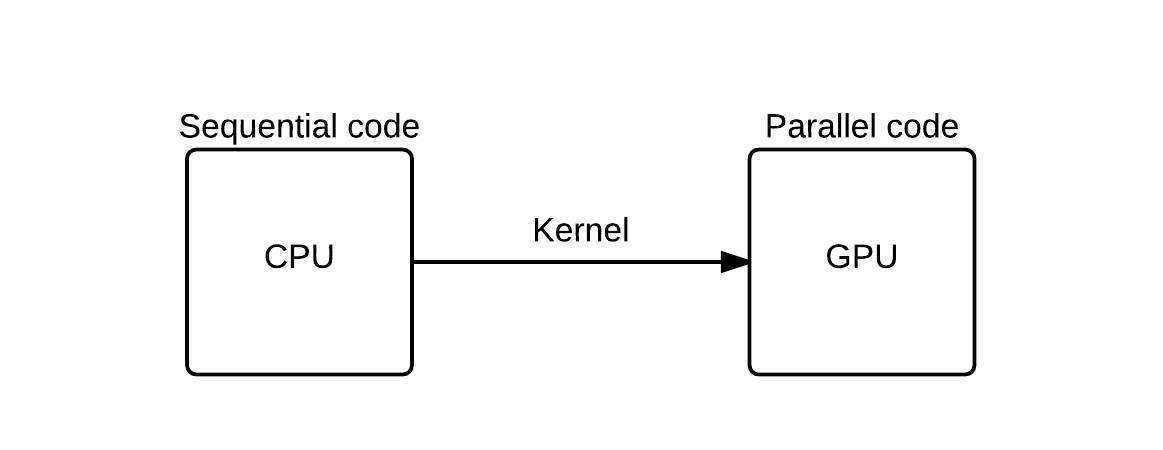
\includegraphics[width=\textwidth]{../system_overview/diagrams/programming_model_cpu_gpu.png}
	\caption{Relationship between CPU and GPU code.}
	\label{fig:programming_model_cpu_gpu}
\end{figure}

\todo{That sentence is a bit dangling and not part of the rest of the chapter. Maybe talk more about CUDA/OpenCL before we start explaining?}
The programming model for Demolicious has been heavily inspired by CUDA and OpenCL, 
and readers with programming experience with those technologies will find much of this chapter familiar.

Many applications can be divided into sequential and parallel parts,
where the characteristics of each part make them benefit from different hardware.
On the Demolicious system, the sequential parts of a program will be run by the CPU, and the parallel parts can be performed by the GPU through kernels.
\todo{Mention SIMT}
A kernel is a simple program meant to be executed by multiple threads.
The kernels are uploaded to the GPU, and then executed when requested by the CPU.
This interaction allows for programs that consist of both parallel and sequential tasks, such as graphics applications.
\todo{Replace last sentence}

\subsection{Kernels}
The GPU can start a massive amount of threads executing the same kernel.
Each thread executing the kernel is assigned a unique thread id.
The thread id can be used to compute memory addresses and make control decisions
to make the threads behave differently even though they are executing the same code. 
\todo{See masking. Do/should we have a subchapter about masking?}

The instruction set is fairly limited.
Most notably, the control flow in kernels is linear, meaning they cannot do any branches or jumps.
Although the kernels don't support diverging control flow,
it's simulated by supporting conditional execution through masking.

\todo{Should we use the term predicated instructions instead? The guy at the presentation was confused when I talked about masking and wondered whether I meant predicated instructions}

Each of the instructions in the instruction set can be executed conditionally by prefixing them with \emph{?}.
Whether a conditional instruction is executed is controlled by a dedicated masking register.
The programmer may use arithmetic and logic operations to manipulate this register (such as the slt instruction in figure \ref{fig:conditional_execution}).
A masked instruction is not executed if the mask register is \textbf{1}.

\begin{figure}[H]
	\centering
	\begin{verbatim}
	  slt $mask, $9, $10 ; Mask if register 9 is less than register 10.
	  add $7, $7, $8 ; This instruction will be executed unconditionally.
	? add $7, $7, $8 ; This instruction will be executed conditionally.
	\end{verbatim}
	\caption{Conditionally zeroing a register.}
	\label{fig:conditional_execution}
\end{figure}

\subsection{Memories}

\begin{figure}[H]
	\centering
	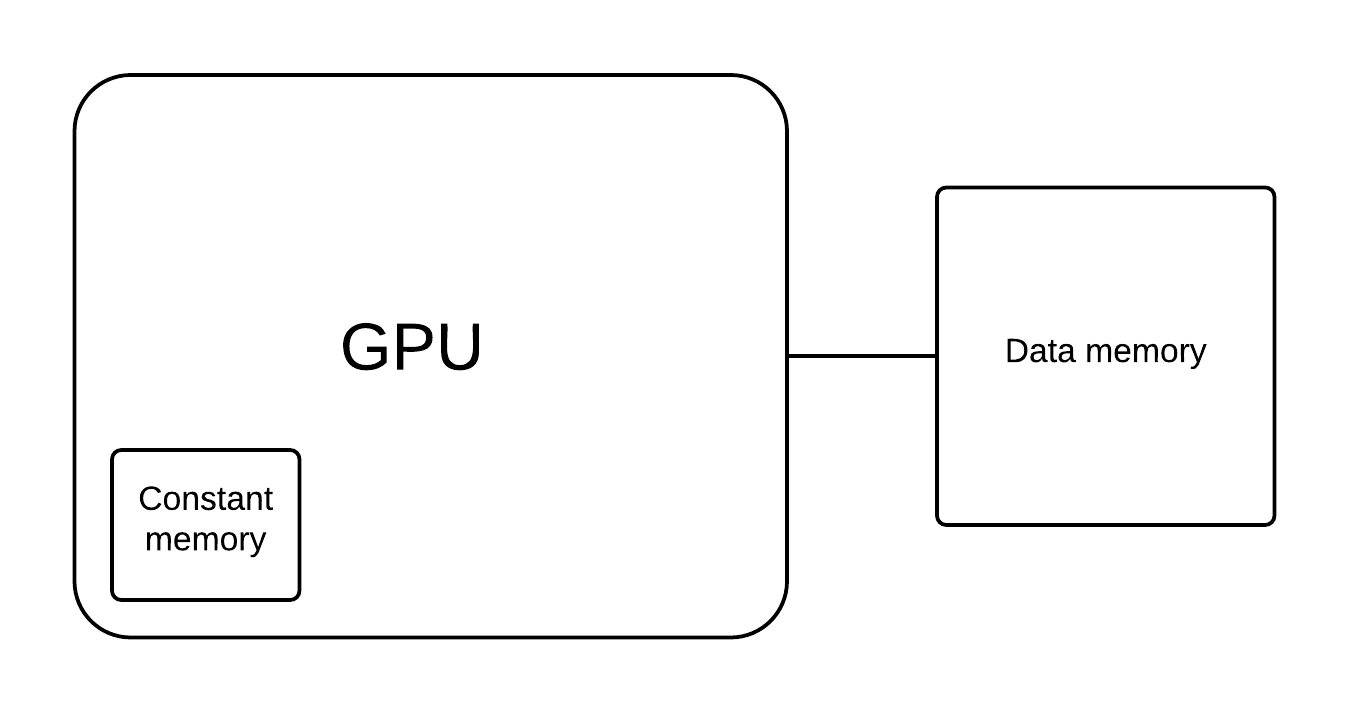
\includegraphics[width=\textwidth]{../system_overview/diagrams/memory_overview.png}
	\caption{Overview of GPU memory architecture.}
	\label{fig:memory_overview}
\end{figure}

The Demolicious system contains two memories that are exposed to the programmer in kernels (figure \ref{fig:memory_overview}).
Data memory is large, but has a relatively high latency.
It is used for storing frame buffers for screen output,
in addition to general data storage for kernels.

The constant memory is a lot faster than the data memory, but is also relatively small.
It is read-only for kernels, meaning only the CPU can write to it.
This makes it suitable for kernel parameters, and enables kernels to be reused with varying output.
For instance, the vertices of a triangle could be stored in constant memory,
and a kernel could read them to render the triangle on screen.
Between kernel runs, the CPU may update the vertices' position, creating animation.

The programmer can access the data memory by using the \emph{load} or \emph{store} instructions.
They require that the memory address and the data is moved into dedicated registers\ref{appendix instruction architecture} in advance.
\todo{add reference to appendix and register overview}

Likewise, there is a dedicated instruction to access the constant memory, named \textit{load constant}.
Because the constant memory is read-only for kernels, there is no \textit{store constant} instruction.

\todo{mention thread finished}

\end{document}